% SC2000 — Chapter 2: Sample Spaces & Events
\chapter{Sample Spaces \& Events}
\label{ch:samplespaces}

\begin{quote}
\emph{``Probability is the logic of uncertainty.''} We cannot predict a single coin toss, but we can describe perfectly the \emph{space} of all possible tosses and assign consistent weights to events. That space and those weights are the foundation of everything that follows.
\end{quote}

\noindent\fbox{\parbox{\dimexpr\linewidth-2\fboxsep-2\fboxrule}{%
\textbf{From zero: sets $\to$ sample spaces.} We assume only sets and counting (Ch.~1). Probability is built as \emph{counting with weights}: favourable over possible, generalised to non-uniform weights via axioms.}}
\vspace{0.4em}

\section*{Learning Outcomes}
After this chapter you will be able to:
\begin{enumerate}[label=(L\arabic*)]
    \item formalise random experiments via sample spaces, events, and set operations;
    \item apply Kolmogorov's axioms and derive basic probability rules;
    \item compute probabilities in equally likely (uniform) models via counting;
    \item use complements, unions, and inclusion--exclusion for events;
    \item distinguish disjoint vs.\ independent events and avoid the confusion.
\end{enumerate}

% ============================================================
\section{Random Experiments and Sample Spaces}
\label{sec:sample-space}
A \emph{random experiment} is any procedure with uncertain outcome but a well-defined set of possibilities.

\begin{definition}[Sample space, event] The \emph{sample space} $\Omega$ is the set of all possible outcomes. A point $\omega\in\Omega$ is an \emph{outcome}. An \emph{event} $A\subseteq\Omega$ is a set of outcomes. The \emph{certain event} is $\Omega$, the \emph{impossible event} is $\emptyset$.
\end{definition}

Examples: coin toss $\Omega=\{H,T\}$; two tosses $\Omega=\{HH,HT,TH,TT\}$; die $\Omega=\{1,\dots,6\}$; packet delay $\Omega=[0,\infty)$ (continuous); infinite coin tosses $\Omega=\{H,T\}^{\infty}$.

\paragraph{Events as sets.} ``At least one head in two tosses'' corresponds to $\{HH,HT,TH\}$. ``Sum of two dice $=7$'' corresponds to $\{(1,6),(2,5),\dots,(6,1)\}$ (6 outcomes out of 36). Set operations: $A\cap B$ (both), $A\cup B$ (at least one), $A^c=\Omega\setminus A$ (not $A$), $A\setminus B$ ($A$ but not $B$).

\begin{figure}[h]
\centering
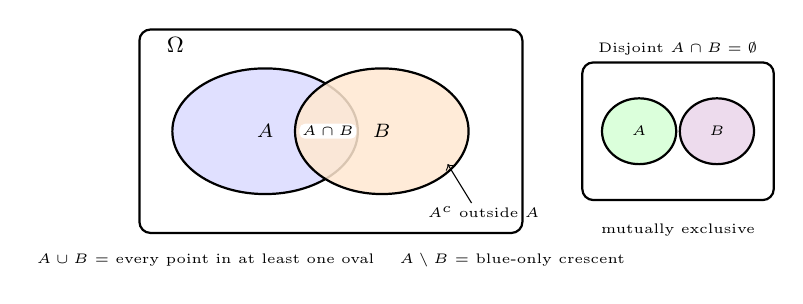
\begin{tikzpicture}[scale=0.76,every node/.style={font=\scriptsize}]
% Venn with sample space rectangle
\draw[thick,rounded corners=4pt] (-3.2,-1.7) rectangle (3.2,1.7);
\node[font=\footnotesize\bfseries] at (-2.6,1.45) {$\Omega$};
% Event A (blue)
\draw[thick,fill=blue!14,fill opacity=0.85] (-1.1,0) ellipse (1.55 and 1.05);
\node at (-1.1,0) {$A$};
% Event B (orange) overlapping
\draw[thick,fill=orange!18,fill opacity=0.85] (0.85,0) ellipse (1.45 and 1.05);
\node at (0.85,0) {$B$};
% intersection label
\node[font=\tiny,fill=white,inner sep=1pt,rounded corners=2pt] at (-0.05,0) {$A\cap B$};
% complement hint
\node[font=\tiny] at (2.55,-1.35) {$A^c$ outside $A$};
\draw[->,thin] (2.35,-1.2)--(1.95,-0.55);
% union annotation
\node[font=\tiny,align=center] at (0,-2.15) {$A\cup B$ = every point in at least one oval \quad $A\setminus B$ = blue-only crescent};
% second mini: disjoint vs overlapping
\begin{scope}[xshift=5.8cm]
\draw[thick,rounded corners=4pt] (-1.6,-1.15) rectangle (1.6,1.15);
\node[font=\tiny] at (0,1.38) {Disjoint $A\cap B=\emptyset$};
\draw[thick,fill=green!14] (-0.65,0) ellipse (0.62 and 0.55);
\draw[thick,fill=violet!14] (0.65,0) ellipse (0.62 and 0.55);
\node[font=\tiny] at (-0.65,0) {$A$}; \node[font=\tiny] at (0.65,0) {$B$};
\node[font=\tiny,align=center] at (0,-1.65) {mutually exclusive};
\end{scope}
\end{tikzpicture}
\caption{Sample space $\Omega$ as a rectangle; events $A,B$ as ovals. Set operations become geometry. Right: disjoint (mutually exclusive) events do not overlap.}
\label{fig:venn-events}
\end{figure}

% ============================================================
\section{Kolmogorov's Axioms}
\label{sec:axioms}
We assign each event a number $P(A)\in[0,1]$ obeying:

\begin{definition}[Probability axioms] A function $P$ on events is a \emph{probability measure} if
\begin{enumerate}[label=(A\arabic*)]
    \item $P(A)\ge0$ for every event $A$;
    \item $P(\Omega)=1$;
    \item \emph{Countable additivity:} if $A_1,A_2,\dots$ are pairwise disjoint, $P(\bigcup_i A_i)=\sum_i P(A_i)$.
\end{enumerate}
\end{definition}

Consequences (prove each from axioms):
\begin{itemize}
    \item $P(\emptyset)=0$, $P(A^c)=1-P(A)$.
    \item If $A\subseteq B$ then $P(A)\le P(B)$ (monotonicity).
    \item $P(A\cup B)=P(A)+P(B)-P(A\cap B)$ (inclusion--exclusion for two events).
    \item $P(A\cup B)\le P(A)+P(B)$ (union bound / Boole's inequality), with equality iff disjoint.
    \item Continuity: if $A_n\uparrow A$ then $P(A_n)\to P(A)$.
\end{itemize}

\begin{example}[Why axioms?] Without (A3), we could assign $P(\{H\})=0.6$, $P(\{T\})=0.6$ for a coin and get $P(\Omega)=1.2\ne1$. Axioms force consistency. They say nothing about \emph{which} numbers---that is modelling.
\end{example}

% ============================================================
\section{Equally Likely Outcomes (Uniform Model)}
\label{sec:uniform}
When $\Omega$ is finite and every outcome is equally likely,
\[
P(A)=\frac{|A|}{|\Omega|}=\frac{\text{\# favourable}}{\text{\# possible}}.
\]
This reduces probability to \emph{counting} (Ch.~1). Verify uniformity is justified (fair coin, well-shuffled deck) before using it!

\begin{example}[Two dice] $\Omega$ has $36$ ordered pairs. $A=\{\text{sum }7\}$ has $6$ outcomes, so $P(A)=6/36=1/6$. $B=\{\text{at least one }6\}$ has $11$ outcomes ($6+6-1$), $P(B)=11/36$.
\end{example}

\begin{example}[Birthday problem preview] With $n$ people and
$365$ days (ignore Feb~29),
$P(\text{all distinct})=365\cdot364\cdots(365-n+1)/365^n$.
For $n=23$, $P(\text{collision})\approx50.7\%$.
\end{example}

\begin{figure}[h]
\centering
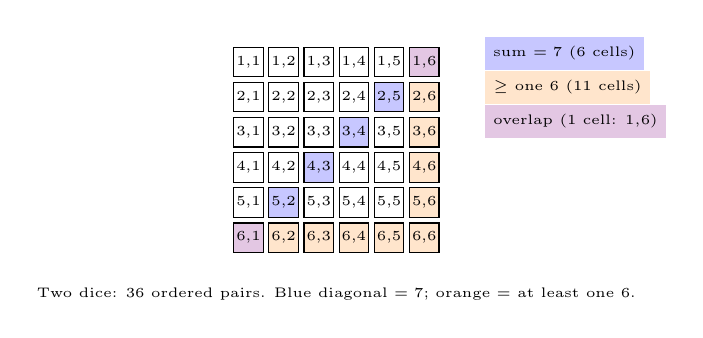
\begin{tikzpicture}[scale=0.72,every node/.style={font=\scriptsize}]
% Grid of 36 dice outcomes, highlight sum=7 diagonal and at-least-one-6
\foreach \r in {0,...,5} {
  \foreach \c in {0,...,5} {
    \pgfmathsetmacro{\x}{\c*0.62}
    \pgfmathsetmacro{\y}{-\r*0.62}
    \pgfmathsetmacro{\s}{\r+\c+2} % sum
    \pgfmathsetmacro{\hasSix}{(\r==5 || \c==5) ? 1 : 0}
    \pgfmathsetmacro{\isSeven}{(\s==7) ? 1 : 0}
    \ifnum\isSeven=1
      \fill[blue!22] (\x-0.26,\y-0.26) rectangle (\x+0.26,\y+0.26);
    \fi
    \ifnum\hasSix=1
      \fill[orange!20] (\x-0.26,\y-0.26) rectangle (\x+0.26,\y+0.26);
      \ifnum\isSeven=1 \fill[violet!22] (\x-0.26,\y-0.26) rectangle (\x+0.26,\y+0.26); \fi
    \fi
    \draw[thin] (\x-0.26,\y-0.26) rectangle (\x+0.26,\y+0.26);
    \node[font=\tiny] at (\x,\y) {\pgfmathtruncatemacro{\a}{\r+1}\pgfmathtruncatemacro{\b}{\c+1}$\a$,$\b$};
  }
}
\node[font=\tiny,anchor=west] at (4.0,0.15) {\colorbox{blue!22}{\strut sum $=7$ (6 cells)}};
\node[font=\tiny,anchor=west] at (4.0,-0.45) {\colorbox{orange!20}{\strut $\ge$ one $6$ (11 cells)}};
\node[font=\tiny,anchor=west] at (4.0,-1.05) {\colorbox{violet!22}{\strut overlap (1 cell: $1{,}6$)}};
\node[font=\tiny,align=center] at (1.55,-4.1) {Two dice: $36$ ordered pairs. Blue diagonal $=7$; orange $=$ at least one $6$.};
\end{tikzpicture}
\caption{Uniform model for two dice: counting favourable cells in the $6\times6$ grid.}
\label{fig:dice-grid}
\end{figure}

% ============================================================
\section{Non-Uniform Models and Continuous Spaces}
\label{sec:nonuniform}
Not every outcome is equally likely. A biased coin: $P(H)=p$, $P(T)=1-p$. A loaded die: arbitrary $p_1,\dots,p_6$ summing to $1$. Axioms still hold; we just assign weights $p(\omega)$ with $\sum_{\omega}p(\omega)=1$ and $P(A)=\sum_{\omega\in A}p(\omega)$.

For continuous $\Omega$ (e.g., $[0,1]$ for a random number), single points have probability $0$; we assign probability to \emph{intervals} via a density. Formally $P([a,b])=\int_a^b f(x)\,dx$ where $f\ge0$, $\int_{\Omega}f=1$. This previews Ch.~4 (random variables).

% ============================================================
\section{Disjoint vs.\ Independent --- A Critical Distinction}
\label{sec:disjoint-independent}

\begin{definition}[Disjoint] $A$ and $B$ are \emph{disjoint} (mutually exclusive) if $A\cap B=\emptyset$.
\end{definition}

Disjoint is a \emph{set} property (no overlap); it forces $P(A\cup B)=P(A)+P(B)$. Independence (Ch.~3) is a \emph{probabilistic} property $P(A\cap B)=P(A)P(B)$ and depends on $P$. Disjoint events with positive probability are \emph{never} independent (if $A\cap B=\emptyset$ then $P(A\cap B)=0\ne P(A)P(B)>0$). Do not confuse them!

\begin{example} Die roll: $A=\{1,2\}$, $B=\{3,4\}$ are disjoint. $C=\{1,3,5\}$ (odd) and $D=\{1,2,3\}$ are not disjoint ($1,3$ overlap) and not independent either ($P(C\cap D)=2/6\ne(3/6)(3/6)$).
\end{example}

% ============================================================
\section{Why Countable Additivity Matters ( countable $\Omega$)}
\label{sec:countable}
Finite additivity $P(A\cup B)=P(A)+P(B)$ for disjoint $A,B$ is not enough for infinite $\Omega$ (e.g., $\Omega=\mathbb{N}$). Countable additivity (A3) lets us sum over countably many disjoint events---needed for geometric distributions $P(X=k)=(1-p)^{k-1}p$ where $\sum_{k\ge1}P(X=k)=1$ is an infinite sum. Without it, paradoxes arise (finitely additive ``probabilities'' that assign $0$ to every singleton yet $1$ to $\mathbb{N}$). For this book, remember: every infinite disjoint union's probability is the sum of the infinite series.

% ============================================================
\section{Computing Probabilities in Code}
\label{sec:code-prob}

\begin{lstlisting}[language=Python]
import math, itertools

# Uniform model: two dice
Omega = list(itertools.product(range(1,7), repeat=2))
def prob(event): return len(event) / len(Omega)

sum7 = [x for x in Omega if sum(x)==7]
at_least_one6 = [x for x in Omega if 6 in x]
print(f"P(sum 7) = {prob(sum7):.4f}")          # 0.1667
print(f"P(>= one 6) = {prob(at_least_one6):.4f}") # 0.3056
# inclusion-exclusion check
both = [x for x in sum7 if 6 in x]
print(len(sum7)+len(at_least_one6)-len(both), len(set(sum7)|set(at_least_one6)))

# Birthday collision for n=23
n, days = 23, 365
p_distinct = math.perm(days, n) / days**n
print(f"P(collision, n=23) = {1-p_distinct:.4f}")  # ~0.507
\end{lstlisting}

% ============================================================
\section{Chapter Notes}
Kolmogorov axiomatised probability in 1933 (\emph{Grundbegriffe}). The rectangle-and-ovals picture is Venn (1880); the distinction disjoint/independent trips up even experienced practitioners. For continuous spaces the axioms extend via measure theory (see Billingsley); computing needs only the intuition: probability as area under a density.

% ============================================================
\section{Exercises}
\label{sec:ch02-exercises}
\begin{enumerate}[label=E2.\arabic*, leftmargin=*, itemsep=0.8em]
\item \textbf{Axioms drill.} From (A1)--(A3) prove:\\
(a) $P(A^c)=1-P(A)$, (b) if $A\subseteq B$ then $P(A)\le P(B)$,\\
(c) $P(A\cup B)=P(A)+P(B)-P(A\cap B)$.\\
Which step uses countable additivity?
\item \textbf{Uniform counting.} A $5$-card hand is dealt from $52$ cards. Compute $P(\text{at least one ace})$ exactly (as a fraction) via the complement. Then compute $P(\text{two pairs})$ and explain the counting.
\item \textbf{Non-uniform.} A biased coin has $P(H)=0.6$. Two independent tosses (independence defined in Ch.~3, assume product rule here). List $\Omega$ with weights $p(\omega)$ and compute $P(\text{at least one }H)$. Why is $P(HH)\ne1/4$?
\item \textbf{Disjoint vs.\ independent.} Give an example of (a) disjoint but not independent events, (b) independent but not disjoint events, (c) events that are neither. Prove disjoint + positive probability $\Rightarrow$ not independent.
\item \textbf{Union bound.} Prove Boole's inequality $P(\bigcup_{i=1}^n A_i)\le\sum_i P(A_i)$ by induction from two-event inclusion--exclusion. When does equality hold? Give a computing use-case (e.g., bounding failure probability of $n$ independent components).
\end{enumerate}
% End of Chapter 2
